\documentclass[11pt]{article}
\usepackage[margin=1in]{geometry}\usepackage{amsmath,amssymb,amsthm,booktabs,graphicx,xcolor,longtable}
\usepackage[numbers,sort&compress]{natbib}
\usepackage[colorlinks=true,linkcolor=blue!50!black,citecolor=blue!50!black,urlcolor=blue!50!black]{hyperref}\usepackage{xurl}\emergencystretch=3em
\usepackage{caption}\captionsetup{font=small,labelfont=bf}\usepackage{placeins}\usepackage{enumitem}
\usepackage[most]{tcolorbox}
\newtcolorbox{insight}[1][]{colback=blue!3!white,colframe=blue!40!black,fonttitle=\bfseries\small,title=#1,boxrule=0.5pt,arc=2pt,left=4pt,right=4pt,top=2pt,bottom=2pt}
\newtheorem{proposition}{Proposition}
\setlist{itemsep=2pt,topsep=3pt}
\renewcommand{\floatpagefraction}{0.85}\renewcommand{\topfraction}{0.9}\renewcommand{\textfraction}{0.08}
\newcommand{\cov}{\mathrm{Cov}}\newcommand{\1}{\mathbb{1}}

\title{How Far Can a Regression Prediction Be Trusted?\\[2pt] \large A Benchmark of Conformal, Distributional and Learned-Coverage Uncertainty Quantification on Nine Engineering and Environmental Datasets}
\author{Danesh Selwal \and Mahesh Pal}
\date{Regression UQ Benchmark v2.0 --- November 2026}
\begin{document}\maketitle
\begin{abstract}Prediction intervals are the simplest honest answer to the question ``how far can this regression prediction be trusted?''. We benchmark more than thirty uncertainty quantification methods, wrapped around nine tuned gradient-boosted, probabilistic and neural regressors, on nine engineering and environmental datasets with 24 to 365 test points. Each method's 90\% interval is checked with a sample-size-aware validity rule and compared on width relative to the spread of the target. Model-based intervals are unreliable: raw quantile regression reaches a median coverage of 58.3\%--90.0\% across datasets with crossing quantiles on most test points, and native NGBoost and PGBM Gaussian intervals are severely over-confident on most datasets. Conformal methods are valid in 1480 of 1557 dataset--model--method cases (95.1\%), with the misses concentrated on two datasets. Among valid methods widths differ by a factor of two or more, and the sharpest valid method changes with the data: jackknife+-after-bootstrap, an online method (FACI, MFCS) or a weighted method (NexCP J+aB). Every number is read from executed Kaggle notebooks released with the code, and each method is explained with its mathematics.\end{abstract}
\tableofcontents
\newpage
\section{Introduction}
Regression models are used in engineering and environmental practice to predict quantities such as concrete strength, pile capacity and
settlement, scour depth, sediment load, streamflow salinity, noise level and water-quality indices. In these applications a prediction is
used to make a decision, and the decision depends on how wrong the prediction could be. A point prediction cannot say this.

Uncertainty quantification (UQ) adds an interval or a distribution to each prediction, and the literature offers dozens of ways to do so.
They differ in what they promise. \emph{Conformal prediction} gives a finite-sample guarantee of marginal coverage under exchangeability
\cite{vovk2005alrw,lei2018distribution,angelopoulos2023gentle}; \emph{weighted} and \emph{online} conformal methods relax that assumption
\cite{barber2023beyond,gibbs2021aci}; \emph{quantile regression} and \emph{predictive distributions} are correct only if the model is
\cite{koenker1978quantile,duan2020ngboost}; and newer methods learn their own coverage level \cite{gauthier2026acp} or extract uncertainty from a
single network \cite{choi2026hcm}. Practitioners rarely see these methods compared on the same small, tabular, real datasets they work with.

This paper runs one fixed pipeline of eight notebooks on nine datasets and asks:
\begin{enumerate}[label=\textbf{Q\arabic*.}]
\item Do model-based intervals (quantile regression, NGBoost, PGBM, IBUG, Treeffuser, CARD) reach their nominal coverage?
\item Do conformal methods keep their promise on real, small datasets, and where do they fail?
\item Among valid methods, which are the sharpest, and is the answer the same on every dataset?
\item What do learned-coverage policies and single-network uncertainty add?
\end{enumerate}
\paragraph{Contributions.} (i) An executed benchmark of $>30$ UQ methods $\times$ 9 base models $\times$ 9 datasets (1800 two-sided intervals), with every executed notebook and raw output released; (ii) a self-contained explanation of the
mathematics of each method and of why its guarantee holds or fails; (iii) a sample-size-aware validity rule and a recommendation rule that turn the
results into a per-dataset choice; (iv) a correctness audit of the original notebooks, with each fix documented. A separate report for each
dataset gives the full detail.

\section{Problem set-up and notation}\label{sec:setup}
We observe training pairs $(X_i,Y_i)$, $i=1,\dots,n$, with features $X_i\in\mathbb R^d$ and a real-valued response
$Y_i$, and want to say something about the response $Y_{n+1}$ of a new point $X_{n+1}$. A \emph{point predictor}
$\hat f$ returns one number $\hat f(X_{n+1})$. An \emph{uncertainty quantification} (UQ) method returns more:
\begin{itemize}
\item a \textbf{prediction interval} $\hat C(x)=[\ell(x),u(x)]$ that should contain the response with probability
$1-\alpha$ (here $1-\alpha=0.9$), or
\item a \textbf{predictive distribution} $\hat F_x$, a full cumulative distribution function for $Y$ given $X=x$, from which
intervals, quantiles and probabilities of exceedance can all be read.
\end{itemize}
Two properties are wanted, and they pull in opposite directions.

\paragraph{Validity (calibration).} The interval should contain the truth as often as it claims:
\begin{equation}\label{eq:marginal}
\Pr\big(Y_{n+1}\in\hat C(X_{n+1})\big)\;\ge\;1-\alpha .
\end{equation}
This is \emph{marginal} coverage: the probability is taken over the random training data \emph{and} the random new point, so it
is an average over the whole population of test points. It does not promise $1-\alpha$ for every value of $x$
(\emph{conditional} coverage, $\Pr(Y\in\hat C(X)\mid X=x)\ge1-\alpha$ for all $x$), which is impossible to guarantee
in finite samples without further assumptions \cite{lei2018distribution}.

\paragraph{Sharpness (efficiency).} Subject to validity, the interval should be as narrow as possible. An interval
$(-\infty,\infty)$ is perfectly valid and useless. We therefore always report coverage \emph{and} width
together, and compare widths only among methods that are valid.

\paragraph{Exchangeability.} Conformal guarantees rely on one assumption: the $n+1$ pairs
$(X_i,Y_i)$, $i=1,\dots,n+1$, are \emph{exchangeable}, meaning their joint distribution does not change when the
pairs are permuted. Independent and identically distributed (i.i.d.) data are exchangeable. Data with a time trend,
or a test set drawn from a different region than the training set, are not.

\paragraph{Notation.} $\alpha$ is the miscoverage level ($\alpha=0.1$ throughout, so intervals target 90\%);
$\hat f$ is a fitted regressor; $s(x,y)$ is a \emph{nonconformity score}, usually the absolute residual
$s(x,y)=|y-\hat f(x)|$; $\lceil\cdot\rceil$ rounds up; $\1\{\cdot\}$ is the indicator function; $\Phi$ and
$\varphi$ are the standard normal CDF and density; $n_{\text{test}}$ is the number of test points.
For a finite list of numbers $v_1,\dots,v_m$ we write $v_{(k)}$ for the $k$-th smallest.

\section{Datasets}\label{sec:data}
\begin{table}[t]\centering\small
\caption{The nine datasets. $p$: number of features; sd: standard deviation of the test target; threshold: lowest coverage accepted as valid (eq.~\ref{eq:valid}).}\label{tab:datasets}
\begin{tabular}{lrrrlrr}\toprule Dataset & Train & Test & $p$ & Target & sd & Threshold\\\midrule
Concrete & 189 & 95 & 7 & \texttt{str} & 10.03 & 0.849\\
Noise & 168 & 60 & 5 & \texttt{Leq} & 15.02 & 0.836\\
Pile & 81 & 24 & 7 & \texttt{Total} & 1.33 & 0.799\\
Pile settlement & 371 & 186 & 8 & \texttt{S\_exp } & 27.20 & 0.864\\
Scour & 154 & 78 & 7 & \texttt{ Scour  } & 1.06 & 0.844\\
Sediment load & 1095 & 365 & 3 & \texttt{St} & 1,235 & 0.874\\
Streamflow & 192 & 96 & 4 & \texttt{TDS} & 197.1 & 0.850\\
Water quality (EWQI) & 47 & 47 & 14 & \texttt{Pre monsoon EWQI } & 57.44 & 0.828\\
Water quality (WQI) & 190 & 82 & 151 & \texttt{WQI} & 72.93 & 0.846\\
\bottomrule\end{tabular}\end{table}
\begin{figure}[t]\centering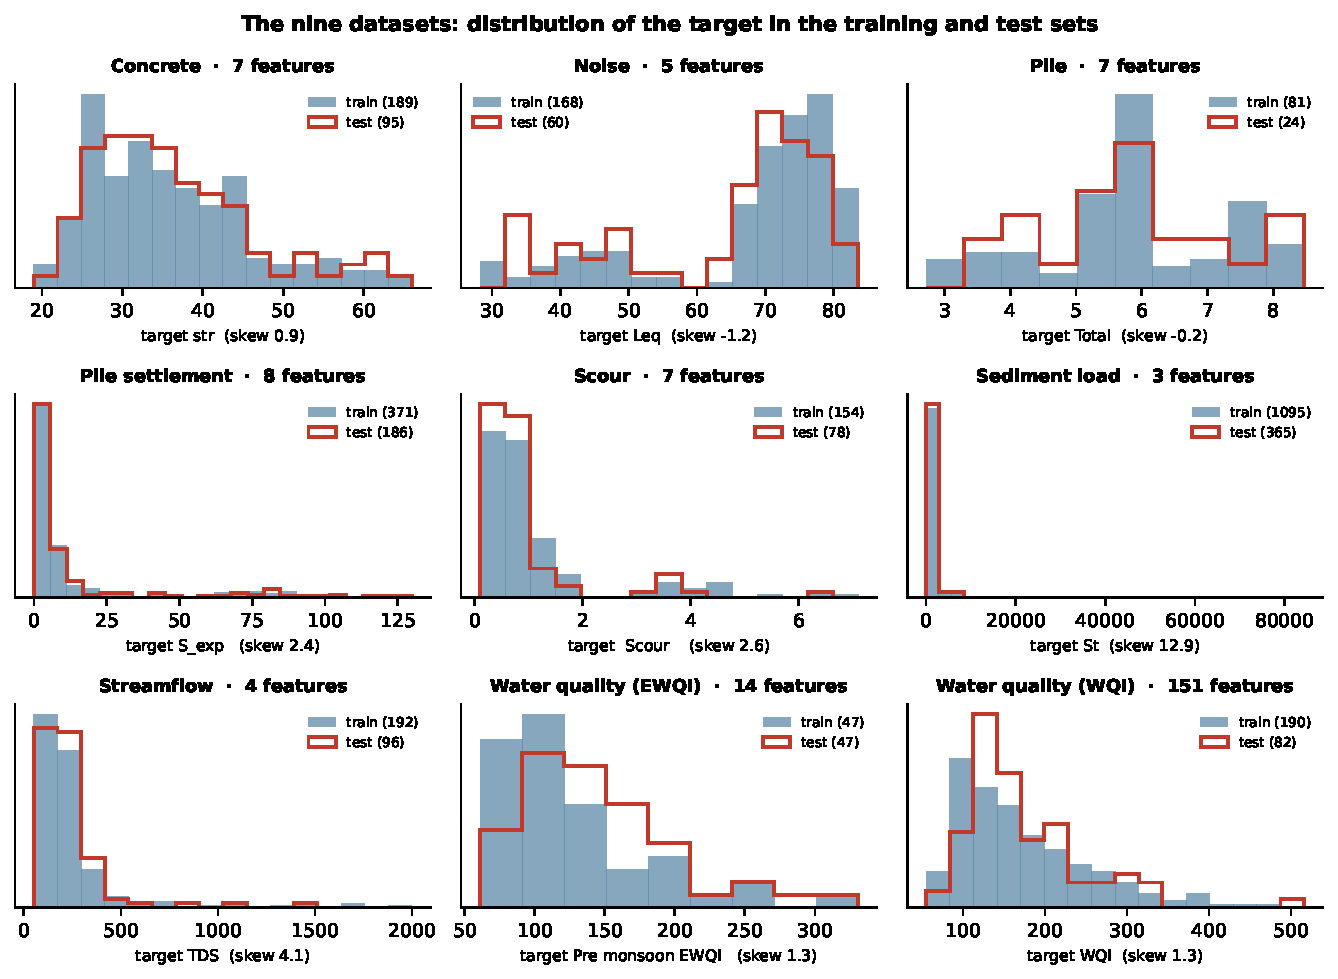
\includegraphics[width=\linewidth]{figures/fig_datasets.pdf}\caption{Target distribution of each dataset on the training (filled) and test (outline) sets.}\label{fig:datasets}\end{figure}
Table~\ref{tab:datasets} and Fig.~\ref{fig:datasets} summarise the nine datasets. They are small (47--1095 training rows) and varied: four
have strongly right-skewed targets (sediment load, streamflow, scour, pile settlement), one has more features than a tree model can use reliably with
its sample size (WQI: 151 features, 190 rows), and two have tiny test sets (pile: 24, EWQI: 47) on which only large departures from 90\% coverage can
be detected. The train/test split is the one supplied with each dataset.

\section{Pipeline and protocol}\label{sec:pipeline}
\begin{figure}[t]\centering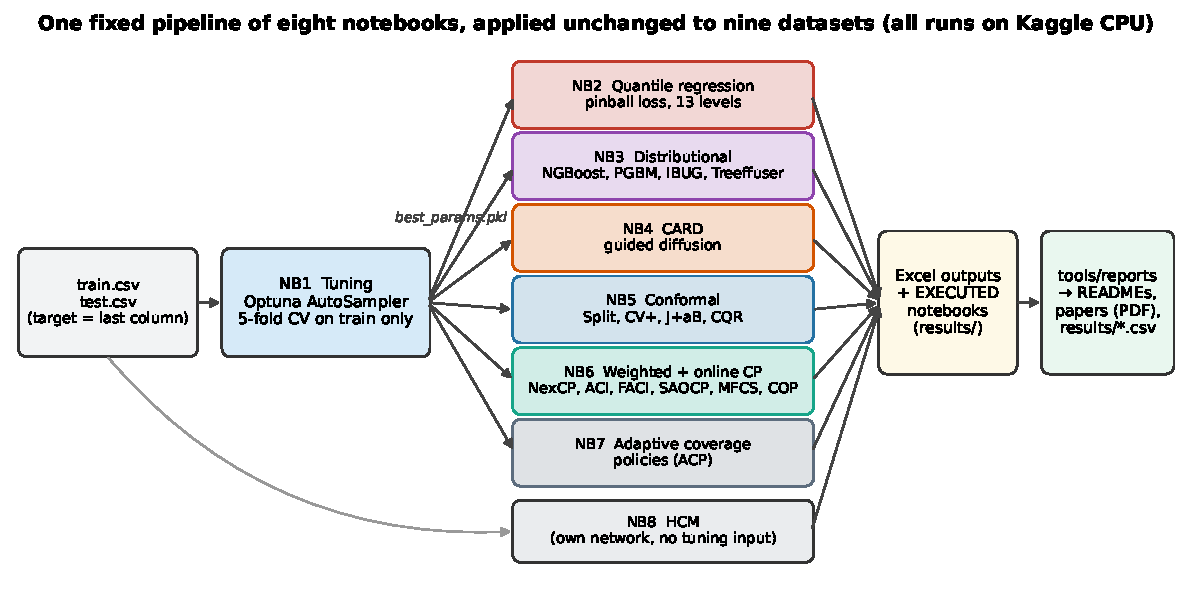
\includegraphics[width=\linewidth]{figures/fig_pipeline.pdf}\caption{The eight-notebook pipeline, run unchanged on every dataset.}\label{fig:pipeline}\end{figure}
Figure~\ref{fig:pipeline} shows the pipeline. Notebook 1 tunes the base models by 5-fold cross-validation on the training set and writes the
settings that notebooks 2--7 load; the test set is used only once, for evaluation. All runs used Kaggle CPU sessions; long notebooks were split into
one job per base model to fit the 12-hour session limit. Two sets of jobs exceeded Kaggle's 12-hour limit and were not re-run (not enough compute): Notebook 6 for TabNet and PGBM on sediment load (where NexCP Full was also switched off for every model) and Notebook 6 for NGBoost and PGBM on pile settlement. These cells are missing, not estimated. The v1.2 notebooks were audited method by method against the original papers
and reference code; every fix is listed in \texttt{docs/CHANGELOG\_FIXES.md}.

\section{Methods}\label{sec:methods}
The pipeline has eight notebooks (Fig.~\ref{fig:pipeline}). This section explains what each method computes and
why it should, or should not, be expected to give 90\% coverage. Each subsection ends with the exact settings used.

\subsection{Base regressors and hyperparameter tuning (NB1)}
Ten regressors are used: random forest \cite{breiman2001rf}, gradient boosting \cite{friedman2001gbm}, histogram
gradient boosting (HistGB, \cite{pedregosa2011sklearn}), XGBoost \cite{chen2016xgboost}, LightGBM \cite{ke2017lightgbm},
CatBoost \cite{prokhorenkova2018catboost}, GPBoost \cite{sigrist2022gpboost}, NGBoost \cite{duan2020ngboost},
PGBM \cite{sprangers2021pgbm} and TabNet \cite{arik2021tabnet}. All but TabNet are tree ensembles; TabNet is an
attention-based neural network for tables. Random forest is used only in tuning; the other nine are the \emph{base
models} that every UQ method wraps.

Each model's hyperparameters $\theta$ are chosen by Optuna \cite{akiba2019optuna} to minimise the 5-fold
cross-validated root mean squared error on the \emph{training set only}:
\begin{equation}
\hat\theta=\arg\min_\theta\;\frac15\sum_{k=1}^5\sqrt{\frac{1}{|I_k|}\sum_{i\in I_k}\big(Y_i-\hat f^{(-k)}_\theta(X_i)\big)^2},
\end{equation}
where $I_k$ is the $k$-th fold and $\hat f^{(-k)}_\theta$ is fitted on the other four folds. The sampler is Optuna's
AutoSampler, which picks a search strategy (for example a tree-structured Parzen estimator) from the search space.
Unpromising trials are stopped early by a \emph{pruner}; each model is tuned with several pruners (median,
Hyperband \cite{li2018hyperband}, Wilcoxon, none) and the setting with the lowest CV error is kept. The selected
settings are written to \texttt{best\_params.pkl} and loaded by every later notebook, so all UQ methods wrap the same
models. The test set is never used for tuning or calibration; it is used once, for the final evaluation.

\begin{insight}[Why this matters]
In v1.2 the tuning objective was the test-set error, so every later coverage number was optimistic. Tuning on
cross-validation only (FIX~1) is a precondition for any honest coverage estimate.
\end{insight}

\subsection{Quantile regression (NB2)}
The $\tau$-quantile $q_\tau(x)$ of $Y$ given $X=x$ minimises the expected \emph{pinball loss}
\cite{koenker1978quantile}
\begin{equation}
\rho_\tau(r)=r\,\big(\tau-\1\{r<0\}\big)=\begin{cases}\tau\,r & r\ge0\\(\tau-1)\,r & r<0\end{cases},\qquad r=y-q .
\end{equation}
\emph{Why this works:} the derivative of $\mathbb E\,\rho_\tau(Y-q)$ with respect to $q$ is $\Pr(Y<q)-\tau$, which is
zero exactly when $q$ is the $\tau$-quantile. Under-predictions are charged $\tau$ per unit and over-predictions
$1-\tau$, so for $\tau=0.95$ the model is pushed up until only 5\% of points lie above it.

Every boosted model (and TabNet, with a pinball loss) is fitted separately for 13 levels
$\tau\in\{0.05,0.1,0.15,0.2,0.3,\dots,0.8,0.85,0.9,0.95\}$. The 90\% interval is $[\hat q_{0.05}(x),\hat q_{0.95}(x)]$.
This interval has \emph{no finite-sample guarantee}: it is correct only if each quantile model is correct, and with a
few hundred points the extreme quantiles are learned from very few observations.

\paragraph{Quantile crossing.} Because each level is a separate model, the predicted quantiles of one point can
be out of order (e.g.\ $\hat q_{0.05}(x)>\hat q_{0.10}(x)$) \cite{chernozhukov2010rearrangement}. We report the
\emph{crossing rate}, the share of test points with at least one inversion, and then sort the 13 values of each
point (monotone rearrangement). Sorting never makes a quantile prediction worse in pinball loss
\cite{chernozhukov2010rearrangement}.

\paragraph{CRPS from quantiles.} The continuous ranked probability score of a predictive CDF $F$ is
\begin{equation}\label{eq:crps}
\mathrm{CRPS}(F,y)=\int_{-\infty}^{\infty}\big(F(z)-\1\{z\ge y\}\big)^2dz
=2\int_0^1\rho_\tau\big(y-F^{-1}(\tau)\big)\,d\tau ,
\end{equation}
the second form showing that CRPS is the pinball loss averaged over all levels \cite{gneiting2007scoring}. With 13 levels
we use $\mathrm{CRPS}\approx2\sum_jw_j\,\rho_{\tau_j}(y-\hat q_{\tau_j})$, where $w_j$ is the share of $[0,1]$ that level $j$
represents ($\sum_jw_j=1$). CRPS is in the units of the target, is \emph{proper} (it is minimised in expectation by the
true distribution) and reduces to the absolute error for a point forecast.

\subsection{Predictive distributions (NB3, NB4)}
These methods output a full distribution $\hat F_x$. Where it is Gaussian, $\hat F_x=\mathcal N(\hat\mu(x),\hat\sigma^2(x))$,
the 90\% interval is $\hat\mu\pm z_{0.95}\hat\sigma$ with $z_{0.95}=1.645$, and the CRPS has the closed form
\begin{equation}\label{eq:crpsgauss}
\mathrm{CRPS}\big(\mathcal N(\mu,\sigma^2),y\big)=\sigma\Big[z\,\big(2\Phi(z)-1\big)+2\varphi(z)-\tfrac{1}{\sqrt\pi}\Big],\qquad z=\frac{y-\mu}{\sigma}.
\end{equation}
\begin{itemize}
\item \textbf{NGBoost} \cite{duan2020ngboost} boosts the parameters $(\mu,\log\sigma)$ of a Gaussian, moving them along the
\emph{natural} gradient of the negative log-likelihood, which makes the step size invariant to how the distribution is
parameterised.
\item \textbf{PGBM} \cite{sprangers2021pgbm} treats each tree leaf weight as a random variable whose mean and variance
are estimated from the gradients and Hessians that fall into the leaf; summing over trees gives $\hat\mu(x)$ and
$\hat\sigma^2(x)$ in one pass.
\item \textbf{IBUG} \cite{brophy2022ibug} wraps any tree ensemble. For a test point it finds the $k$ training points that
share the most leaves with it (highest \emph{affinity}), and uses the spread of their targets as $\hat\sigma(x)$; the
mean comes from the ensemble. We use IBUG with XGBoost and LightGBM.
\item \textbf{Treeffuser} \cite{beltranvelez2024treeffuser} learns a conditional diffusion model whose score function is
estimated by gradient-boosted trees; samples from the reverse diffusion are non-parametric draws from $\hat F_x$.
\item \textbf{CARD} \cite{han2022card} (NB4) is a classification-and-regression diffusion model guided by a point predictor
$\hat f(x)$. The forward process adds noise while drifting towards the guide:
\begin{equation}
y_t=\sqrt{\bar\alpha_t}\,y_0+\big(1-\sqrt{\bar\alpha_t}\big)\hat f(x)+\sqrt{1-\bar\alpha_t}\,\varepsilon,\qquad\varepsilon\sim\mathcal N(0,1),
\end{equation}
with $\bar\alpha_t=\prod_{s\le t}(1-\beta_s)$ and a linear schedule $\beta_1=10^{-4},\dots,\beta_T=0.02$, $T=1000$. A network
$\varepsilon_\theta(x,y_t,\hat f(x),t)$ is trained to predict the noise, $\min\mathbb E\|\varepsilon-\varepsilon_\theta\|^2$
\cite{ho2020ddpm}, and the reverse process turns pure noise centred on $\hat f(x)$ into samples of $Y\mid x$. Each of the
nine tuned models is used once as the guide; 1000 samples per test point are drawn (official settings: 5000 epochs,
batch 32, learning rate $10^{-3}$, EMA of the weights with warm-up).
\end{itemize}
For sample-based methods (Treeffuser, CARD) we summarise the samples by their mean and standard deviation and report the
Gaussian CRPS~\eqref{eq:crpsgauss} and Gaussian 90\% interval, so that every distributional method is scored the same way.
The notebooks also report the negative log-likelihood, the Hersbach decomposition of CRPS into reliability, resolution and
uncertainty \cite{hersbach2000crps}, and the probability integral transform $\mathrm{PIT}=\hat F_X(Y)$, which is uniform on
$[0,1]$ for a calibrated forecast \cite{gneiting2007sharpness,kuleshov2018calibrated}. A U-shaped PIT histogram means the
distributions are too narrow (over-confident); a hump means they are too wide.

\begin{insight}[What to expect]
None of these distributions comes with a coverage guarantee. A Gaussian assumption fails when errors are skewed or
heavy-tailed, and a $\hat\sigma(x)$ fitted on training data is typically too small, because training residuals are
smaller than test residuals. Their intervals are therefore a \emph{test} of the model, not a guarantee.
\end{insight}

\subsection{Split, cross and bootstrap conformal prediction (NB5)}
Conformal prediction \cite{vovk2005alrw,lei2018distribution,angelopoulos2023gentle} turns any point predictor into an
interval with a finite-sample guarantee. Box~1 in the repository README illustrates the three steps.

\paragraph{Split conformal (SCP).} Split the training data into a fitting part and a calibration part
$\mathcal C$ with $m=|\mathcal C|$ points. Fit $\hat f$ on the first part, compute scores $s_i=|Y_i-\hat f(X_i)|$ on
$\mathcal C$, and set
\begin{equation}\label{eq:scp}
\hat q=s_{(k)},\quad k=\big\lceil(m+1)(1-\alpha)\big\rceil,\qquad \hat C(x)=\big[\hat f(x)-\hat q,\;\hat f(x)+\hat q\big].
\end{equation}
\begin{proposition}[Coverage of split conformal]
If the calibration pairs and the test pair are exchangeable, $\Pr(Y_{n+1}\in\hat C(X_{n+1}))\ge1-\alpha$. If the scores
have no ties, also $\Pr(Y_{n+1}\in\hat C(X_{n+1}))\le1-\alpha+\frac1{m+1}$.
\end{proposition}
\emph{Why.} $\hat f$ was fitted without the calibration and test points, so the $m+1$ scores $s_1,\dots,s_m,s_{n+1}$ are
exchangeable. The rank of $s_{n+1}$ among them is then uniform on $\{1,\dots,m+1\}$, and $Y_{n+1}\in\hat C$ exactly when
$s_{n+1}\le s_{(k)}$, which happens with probability $k/(m+1)\ge1-\alpha$. The ``$+1$'' accounts for the test point
itself. Nothing is assumed about the model or the noise; a poor model gives a valid but wide interval.

\emph{Settings.} MAPIE \cite{taquet2022mapie}: one seeded random half of the training rows fits the model, the other half
calibrates. PUNCC \cite{mendil2023puncc}: its own split. Both use $\alpha=0.1$.

\paragraph{CV+ and jackknife+-after-bootstrap (J+aB).} Split conformal wastes half the data on calibration. CV+
\cite{barber2021jackknife} fits $K$ models $\hat f^{(-k)}$, each without fold $k$, and scores every training point
with the model that did not see it: $R_i=|Y_i-\hat f^{(-k(i))}(X_i)|$. The interval is
\begin{equation}\label{eq:cvplus}
\hat C(x)=\Big[\,\hat q^-_{\alpha}\big\{\hat f^{(-k(i))}(x)-R_i\big\},\;\hat q^+_{\alpha}\big\{\hat f^{(-k(i))}(x)+R_i\big\}\Big],
\end{equation}
where $\hat q^-_\alpha$ is the $\lfloor\alpha(n+1)\rfloor$-th smallest and $\hat q^+_\alpha$ the
$\lceil(1-\alpha)(n+1)\rceil$-th smallest of the $n$ values. Its guarantee is weaker on paper, $1-2\alpha$ (up to a small
term for $K$-fold CV+), but in practice coverage is close to $1-\alpha$ and the interval narrower, because every point
is used both to fit and to calibrate. J+aB \cite{kim2020jab} replaces the folds by $B$ bootstrap samples: $R_i$ uses the
average of the models whose bootstrap sample did not contain $i$ (out-of-bag), and the test prediction aggregates the same
models. \emph{Settings:} $K=5$; J+aB with 50 resamplings (MAPIE \texttt{method="plus"}).

\paragraph{Conformalised quantile regression (CQR).} Symmetric intervals $\hat f\pm\hat q$ have the same width everywhere.
CQR \cite{romano2019cqr} starts from quantile models $\hat q_{\alpha/2},\hat q_{1-\alpha/2}$, whose band already adapts to
$x$, and corrects it with the score
\begin{equation}
s_i=\max\big\{\hat q_{\alpha/2}(X_i)-Y_i,\;Y_i-\hat q_{1-\alpha/2}(X_i)\big\},\qquad
\hat C(x)=\big[\hat q_{\alpha/2}(x)-\hat q,\;\hat q_{1-\alpha/2}(x)+\hat q\big],
\end{equation}
with $\hat q$ from~\eqref{eq:scp}. The score is negative when the point is inside the band, so $\hat q$ can shrink an
over-wide band as well as widen a narrow one; the guarantee is that of split conformal. \emph{Settings:} PUNCC CQR with
native quantile losses (LightGBM, GPBoost, XGBoost, Gradient Boosting, CatBoost, TabNet) or distribution quantiles (NGBoost, PGBM).

\subsection{Weighted conformal prediction: NexCP (NB6)}
When the data drift, old calibration points describe the new point less well. Non-exchangeable conformal prediction
(NexCP, \cite{barber2023beyond}) gives each calibration score a fixed weight $w_i\in[0,1]$ chosen \emph{before} seeing
the data, and uses the weighted quantile
\begin{equation}
\hat q=\mathrm{Quantile}_{1-\alpha}\Big(\sum_{i=1}^n\tilde w_i\,\delta_{s_i}+\tilde w_{n+1}\,\delta_{+\infty}\Big),\qquad
\tilde w_i=\frac{w_i}{\sum_{j=1}^nw_j+1},\;\tilde w_{n+1}=\frac{1}{\sum_jw_j+1},
\end{equation}
where $\delta_v$ is a point mass at $v$. The mass at $+\infty$ plays the role of the ``$+1$'' in~\eqref{eq:scp}. With
$w_i=\rho^{\,n+1-i}$ (here $\rho=0.99$) recent points count more. The guarantee degrades gracefully:
\begin{equation}
\Pr\big(Y_{n+1}\in\hat C(X_{n+1})\big)\;\ge\;1-\alpha-\sum_{i=1}^n\tilde w_i\,d_{\mathrm{TV}}\big(Z,Z^{i}\big),
\end{equation}
where $d_{\mathrm{TV}}(Z,Z^i)$ measures how much the data change when point $i$ is swapped with the test point. If the data are
exchangeable every term is zero and~\eqref{eq:marginal} holds; under drift, down-weighting old points keeps the gap small.
NexCP is run in four forms: \emph{Split} (out-of-fold residuals as scores), \emph{CV+} and \emph{J+aB} (weighted
versions of~\eqref{eq:cvplus}), and \emph{Full} conformal, which for each test point refits the model on the training data
plus a candidate $(x,y)$ for 50 values of $y$ on a grid and keeps the values of $y$ that conform. If the weighted quantile is
$+\infty$ the interval is capped at the largest residual and flagged; if a Full interval reaches the edge of its grid the width
is a lower bound and the method is not ranked (marked $\dagger$).

\subsection{Online conformal prediction (NB6)}
Online methods treat the test set as a \emph{stream}: the interval for point $t$ is issued, then $Y_t$ is revealed and used to
update the next interval. They do not need exchangeability; instead they guarantee that the \emph{long-run average}
miscoverage is close to $\alpha$, even under arbitrary distribution shift. Every method here starts from 5-fold out-of-fold
training residuals and issues each interval \emph{before} its own error is used (no look-ahead).

\paragraph{ACI.} Adaptive conformal inference \cite{gibbs2021aci} adjusts the level it asks for:
\begin{equation}\label{eq:aci}
\alpha_{t+1}=\alpha_t+\gamma\,(\alpha-\mathrm{err}_t),\qquad \mathrm{err}_t=\1\{Y_t\notin\hat C_t(X_t)\},
\end{equation}
and $\hat C_t=\hat f(x)\pm\hat q_t$ uses the $(1-\alpha_t)$ quantile of the out-of-fold training residuals plus the test
residuals revealed so far. After a miss ($\mathrm{err}_t=1$) the level $\alpha_t$ drops, so the next
interval is wider; after a hit it rises slightly. Summing~\eqref{eq:aci} over $t$ gives
$\big|\frac1T\sum_{t=1}^T\mathrm{err}_t-\alpha\big|\le\frac{\max(\alpha_1,1-\alpha_1)+\gamma}{\gamma T}$, so the average
miscoverage converges to $\alpha$ for any data sequence. \emph{Settings:} $\gamma=0.005$.

\paragraph{FACI.} The best $\gamma$ is unknown. Fully adaptive conformal inference \cite{gibbs2024faci} runs ACI for a grid of
$\gamma$ values ($0.001\cdot2^k$, $k=0,\dots,7$) as experts and combines their levels with exponential weights based on each
expert's pinball loss (reference settings, interval length $I=100$).

\paragraph{SF-OGD and SAOCP.} Instead of the level, these methods learn the radius $q_t$ directly by online gradient descent
on the pinball loss of the scores,
\begin{equation}
q_{t+1}=q_t-\eta\,\frac{\nabla_t}{\sqrt{\sum_{s\le t}\nabla_s^2}},\qquad \nabla_t=\alpha-\1\{s_t>q_t\},
\end{equation}
so $q$ grows after a miss and shrinks slowly after a hit; the scale-free step needs no tuning of the learning rate to the
units of $Y$ \cite{orabona2018scalefree} ($\eta$ is the largest calibration residual, as in the reference code, and both methods
are warm-started on the calibration residuals). SAOCP \cite{bhatnagar2023saocp} runs SF-OGD experts started at different times and
combines them by coin betting (expert lifetime 8), which gives low regret on \emph{every} time interval and lets it react faster to a change.

\paragraph{Online split, CV+, J+aB and MFCS.} \emph{Online split} (and \emph{MFCS Split}, identical in the code) uses a fixed
radius, the conformal quantile of the out-of-fold training residuals. \emph{Online CV+} and \emph{Online J+aB} apply~\eqref{eq:cvplus}
and add each revealed test residual to the calibration set. \emph{MFCS Full} refits the model on the training data plus all test
points already revealed, and takes its radius from the out-of-fold residuals of that refit; it is the only method that also
updates the point prediction with past test labels. (MFCS has no published reference; it is kept as written in the original
notebooks.)

\paragraph{COP.} Distribution-informed online conformal prediction \cite{hu2026cop} runs the plain online quantile update
$\tilde q_{t+1}=\tilde q_t-\eta_t g_t$, with $g_t=\alpha$ after a hit and $g_t=-(1-\alpha)$ after a miss, and adds an
\emph{optimistic} correction that looks at the empirical distribution $\hat F_t$ of the last $T_{\text{burnin}}$ scores:
\begin{equation}
\tilde g_t=\hat F_t\big(\tilde q_t-\eta_tg_t\big)-(1-\alpha),\qquad q_{t+1}=\max\big(0,\;\tilde q_{t+1}-c\,\eta_t\,\tilde g_t\big).
\end{equation}
In words: if the step about to be taken would already put more than $1-\alpha$ of the recent scores below the radius, the
correction pulls it back, and vice versa, so the radius anticipates where the coverage is heading. The learning rate is
$\eta_t=\eta\cdot(\max-\min)$ of the recent scores, as in the official code. \emph{Settings:} $\eta=0.05$, $c=0.5$, start value the
90\% quantile of the out-of-fold training residuals, $T_{\text{burnin}}$ set from the test-set size (FIX D5).

\begin{insight}[Reading online results]
Online methods use the labels of earlier test points. Their coverage is an average over the stream and their width can
shrink as they learn, which is legitimate when labels really do arrive one by one (monitoring, forecasting). On a static test set
the order of the rows matters; we use the stored order.
\end{insight}

\subsection{Extreme conformal prediction (NB6)}
For a high level the empirical quantile is the largest residual, and it cannot extrapolate. Extreme CP \cite{pasche2025extreme}
fits a generalised Pareto distribution (GPD) \cite{pickands1975gpd} to the exceedances $s_i-u$ of the signed scores
$s_i=Y_i-\hat f(X_i)$ over a high threshold $u$,
\begin{equation}
\Pr(s-u>z\mid s>u)\approx\Big(1+\frac{\xi z}{\sigma}\Big)^{-1/\xi},
\end{equation}
and inverts it for the required level; the procedure is repeated for thresholds at the 0.80--0.99 quantiles (keeping at least 10
exceedances) and the largest bound is used. The result is a \emph{one-sided} bound $Y\le\hat f(x)+\hat q$, so its coverage is
$\Pr(Y\le\hat f+\hat q)$ and it is reported separately from the two-sided intervals.

\subsection{Adaptive coverage policies (NB7)}
All methods above fix $\alpha$ in advance. ACP \cite{gauthier2026acp} lets a small network (AlphaNet: 32 ReLU units, sigmoid
output) choose a level $\tilde\alpha(x)$ for each test point, trading width against coverage through the loss
$\text{width}+\lambda\,\tilde\alpha$ ($\lambda=50$ reported; $\lambda\in\{10,20,50\}$ compared). Validity for a data-dependent level
comes from conformal \emph{e-values} \cite{vovk2021evalues,gauthier2025evalues}: with calibration scores $s_1,\dots,s_n$ the
candidate $y$ is excluded when
\begin{equation}
e(y)=\frac{(n+1)\,s(x,y)}{\sum_{i=1}^ns_i+s(x,y)}\;\ge\;\frac1{\tilde\alpha(x)}
\quad\Longleftrightarrow\quad s(x,y)\ge\frac{\sum_is_i}{\tilde\alpha(x)(n+1)-1},
\end{equation}
so the set is $\hat f(x)\pm\sum_is_i/(\tilde\alpha(n+1)-1)$. The guarantee is $\mathbb E\big[\1\{Y\notin\hat C\}/\tilde\alpha(X)\big]\le1$:
coverage must be compared with the \emph{learned} target $1-\tilde\alpha$, not with 90\%. If the policy pushes $\tilde\alpha$ to its
upper limit (0.999) for every point, the target coverage is 0.1\%, every set has the same width, and the learned level carries no
information; we flag such models as \emph{saturated}.

\subsection{Hyperspherical confidence mapping (NB8)}
HCM \cite{choi2026hcm} is a single, sampling-free network. The scalar target is lifted to $\mathbf y=(y,y)\in\mathbb R^2$ and
split into a magnitude $R=\|\mathbf y\|$ and a unit direction $\mathbf d=\mathbf y/R$. A network with three hidden layers of 20
units predicts $\hat R$ and $\hat{\mathbf d}$ with the symmetric loss
$\mathrm{MSE}(\hat R\,\mathbf d,\mathbf y)+\mathrm{MSE}(R\,\hat{\mathbf d},\mathbf y)$. At test time the predicted direction should lie on the
unit circle; how far it falls off is the uncertainty,
\begin{equation}
\hat\sigma_{\text{raw}}(x)=\sqrt{\big|\,\|\hat{\mathbf d}(x)\|^2-1\big|}\;|\hat R(x)|,
\end{equation}
and a single scale factor is fitted on a validation split so that $\pm1,2,3\,\hat\sigma$ cover 68/95/99.7\%. We report the 95\%
interval, the coverage at $1,2,3\sigma$, and the Spearman correlation between $|y-\hat y|$ and $\hat\sigma$ (positive means the
network knows when it is wrong).

\section{Evaluation protocol}\label{sec:eval}
\paragraph{Coverage and width.} For an interval method and base model, the empirical coverage on the test set is
$\hat c=\frac1{n_{\text{test}}}\sum_{t}\1\{\ell(X_t)\le Y_t\le u(X_t)\}$ and the mean width is
$\bar w=\frac1{n_{\text{test}}}\sum_t\big(u(X_t)-\ell(X_t)\big)$. To compare datasets with different units we also report the
\emph{relative width} $\bar w/\mathrm{sd}(Y_{\text{test}})$: a relative width of 1 means the interval is as wide as one standard
deviation of the target, and an interval that ignored $x$ altogether would need about $2\times1.645=3.3$ for a Gaussian target.

\paragraph{When is a coverage ``valid''?} Even a perfect 90\% method will not cover exactly 90\% of a finite test set. If each test
point is covered independently with probability $0.9$, then $n_{\text{test}}\hat c\sim\mathrm{Binomial}(n_{\text{test}},0.9)$, so
$\hat c$ has standard error $\sqrt{0.9\cdot0.1/n_{\text{test}}}$. We call a method \emph{valid} when $\hat c$ is not significantly
below 90\% in a one-sided test at the 5\% level:
\begin{equation}\label{eq:valid}
\hat c\;\ge\;0.9-1.645\sqrt{\frac{0.09}{n_{\text{test}}}} .
\end{equation}
The test is approximate (online methods produce dependent errors, and many methods are tested at once), so it is used as a
screening rule, not a formal decision.

\paragraph{Recommended method.} A method wraps up to nine base models. It is \emph{recommended} on a dataset if it is the
narrowest method (median relative width over models) among those that are valid for at least 75\% of the models they ran on,
ran on at least three models, and have no width that is a lower bound. Extreme CP (one-sided), ACP (learned level) and HCM (95\%,
own network) are discussed separately.

\paragraph{Scores for distributions.} CRPS (eqs.~\ref{eq:crps}--\ref{eq:crpsgauss}; lower is better, in target units), the negative
log-likelihood, PIT diagnostics and, for HCM, the Spearman correlation between absolute error and predicted spread.

\begin{figure}[h]\centering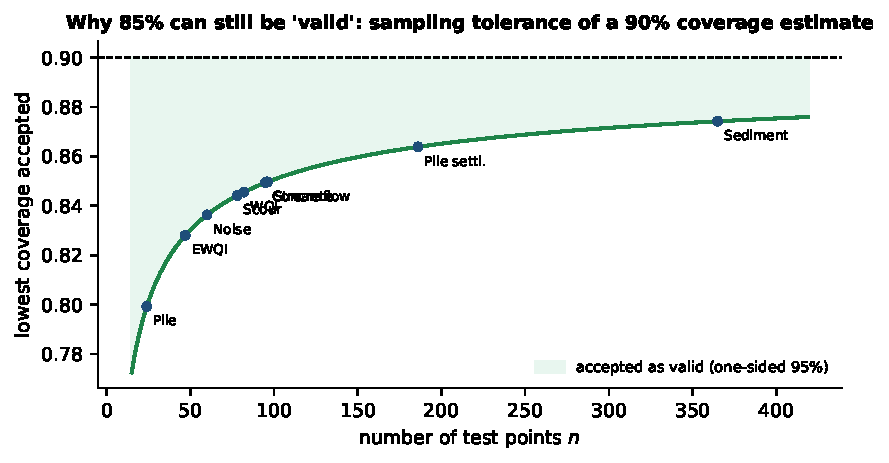
\includegraphics[width=0.75\linewidth]{figures/fig_validity_tolerance.pdf}\caption{Lowest coverage accepted as valid, eq.~\eqref{eq:valid}, as a function of the test-set size, with the nine datasets marked.}\label{fig:tol}\end{figure}
\begin{figure}[h]\centering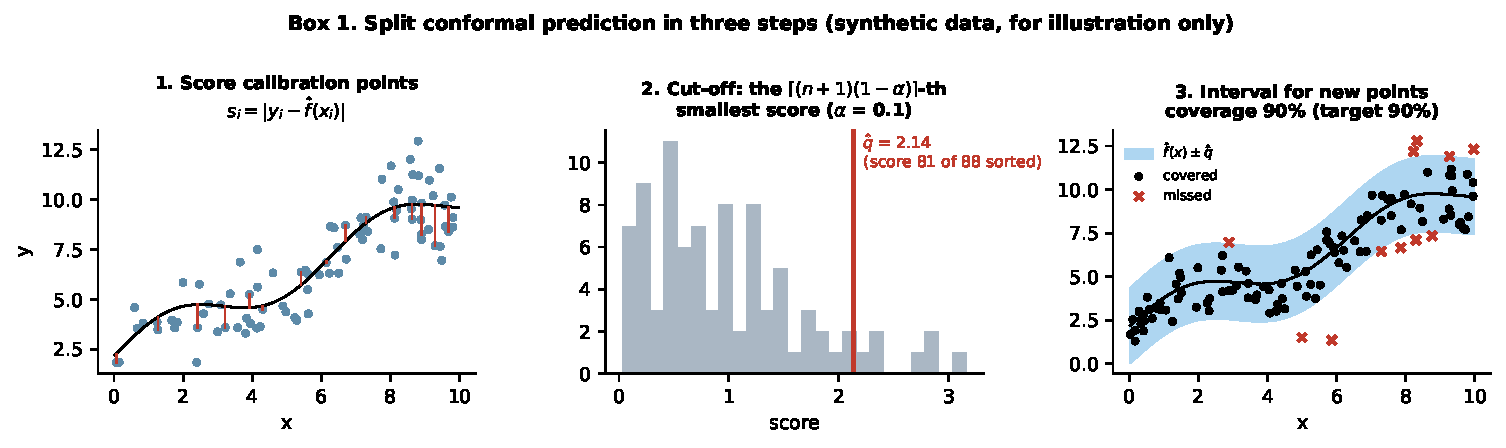
\includegraphics[width=\linewidth]{figures/fig_conformal_explainer.pdf}\caption{Split conformal prediction in three steps on synthetic data: score, cut-off, interval.}\label{fig:explainer}\end{figure}

\section{Results}\label{sec:results}
\subsection{Point accuracy}
\begin{table}[t]\centering\small
\caption{Point accuracy. Best model by 5-fold CV (training set) and best model on the test set; last column: best test RMSE divided by the test-target standard deviation.}\label{tab:acc}
\begin{tabular}{lllllr}\toprule Dataset & Best (CV) & its test RMSE & Best (test) & RMSE & RMSE/sd\\\midrule
Concrete & CatBoost & 2.99 & HistGB & 2.81 & 0.28\\
Noise & LightGBM & 4.06 & GPBoost & 3.39 & 0.23\\
Pile & LightGBM & 0.761 & RandomForest & 0.439 & 0.33\\
Pile settlement & GPBoost & 11.41 & LightGBM & 10.24 & 0.38\\
Scour & XGBoost & 0.404 & PGBM & 0.311 & 0.29\\
Sediment load & TabNet & 728.5 & GradientBoosting & 328.6 & 0.27\\
Streamflow & GradientBoosting & 115.4 & GPBoost & 109.2 & 0.55\\
Water quality (EWQI) & XGBoost & 20.34 & GPBoost & 17.95 & 0.31\\
Water quality (WQI) & XGBoost & 28.74 & CatBoost & 27.16 & 0.37\\
\bottomrule\end{tabular}\end{table}
Table~\ref{tab:acc} shows that the best model differs between datasets and that the CV choice is often, but not always, the best on the test set.
The tree ensembles are close to each other on every dataset; the differences between UQ methods are much larger than the differences between the
boosted base models, which is why the rest of the paper aggregates over base models.

\subsection{Q1: model-based intervals do not reach their nominal coverage}
\begin{table}[t]\centering\small
\caption{Coverage of the model-based 90\% intervals (median over base models where several). Crossing: median share of test points with crossing quantiles.}\label{tab:modelbased}
\resizebox{\textwidth}{!}{\begin{tabular}{lrrrrrrr}\toprule Dataset & QR & Crossing & NGBoost & PGBM & IBUG & Treeffuser & CARD\\\midrule
Concrete & 79.0\% & 97.9\% & 33.7\% & 21.1\% & 91.1\% & 100.0\% & 50.5\%\\
Noise & 90.0\% & 100.0\% & 86.7\% & 6.7\% & 94.2\% & 100.0\% & 70.0\%\\
Pile & 58.3\% & 100.0\% & 0.0\% & 41.7\% & 100.0\% & 100.0\% & 20.8\%\\
Pile settlement & 82.8\% & 99.5\% & 61.3\% & 8.1\% & 96.0\% & 96.8\% & 61.3\%\\
Scour & 84.6\% & 97.4\% & 65.4\% & 100.0\% & 92.9\% & 100.0\% & 74.4\%\\
Sediment load & 81.1\% & 89.9\% & 85.8\% & 6.6\% & 98.5\% & 100.0\% & 94.2\%\\
Streamflow & 86.5\% & 57.3\% & 89.6\% & 16.7\% & 90.6\% & 100.0\% & 78.1\%\\
Water quality (EWQI) & 66.0\% & 100.0\% & 0.0\% & 2.1\% & 95.7\% & 100.0\% & 34.0\%\\
Water quality (WQI) & 79.3\% & 100.0\% & 1.2\% & 14.6\% & 79.9\% & 100.0\% & 25.6\%\\
\bottomrule\end{tabular}}\end{table}
\begin{figure}[t]\centering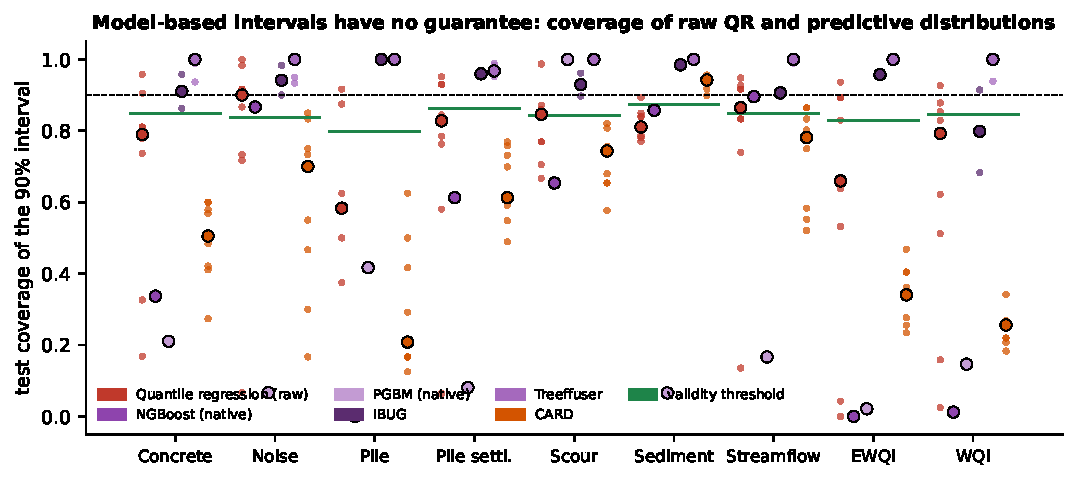
\includegraphics[width=\linewidth]{figures/fig_model_based_coverage.pdf}\caption{Coverage of the model-based 90\% intervals on each dataset. Small dots: individual base models; large dots: median; green bar: validity threshold.}\label{fig:modelbased}\end{figure}
\paragraph{How to read it.} In Fig.~\ref{fig:modelbased} each colour is one method; a method is reliable if its dots sit at or above the green bar
of every dataset. \paragraph{What it shows.}
\begin{itemize}
\item \textbf{Raw quantile regression undercovers}: its median coverage is below the threshold on 6 of nine datasets, and the separately fitted quantiles cross on most test points of almost every dataset (Table~\ref{tab:modelbased}).
\item \textbf{Native NGBoost and PGBM Gaussians are over-confident}: their $\hat\sigma$ is far too small on most datasets (PGBM covers 2--42\% on eight of nine). Their PIT histograms are U-shaped (under-dispersed).
\item \textbf{IBUG and Treeffuser go the other way}: IBUG is usually close to or above 90\%; Treeffuser covers almost everything with very wide intervals.
\item \textbf{CARD} is sharp but undercovers on most datasets; it reaches the target only on the large sediment-load dataset.
\end{itemize}
\begin{insight}[Takeaway Q1]
A predictive distribution that scores well on CRPS can still give a badly calibrated interval. Without a calibration step, no model-based method is reliable across datasets.
\end{insight}

\subsection{Q2: conformal methods are valid almost everywhere}
\begin{table}[t]\centering\small
\caption{All model $\times$ method $\times$ dataset intervals pooled by family: number of intervals, share valid and median relative width.}\label{tab:family}
\begin{tabular}{lrrr}\toprule Family & Intervals & Valid & Median width/sd\\\midrule
Quantile regression & 81 & 38.3\% & 0.91\\
Distributional & 81 & 80.2\% & 2.24\\
CARD & 81 & 14.8\% & 0.26\\
Conformal (MAPIE/PUNCC) & 486 & 94.0\% & 1.48\\
Weighted conformal (NexCP) & 301 & 94.4\% & 1.47\\
Online conformal & 693 & 95.7\% & 1.40\\
COP & 77 & 98.7\% & 1.34\\
\bottomrule\end{tabular}\end{table}
\begin{figure}[t]\centering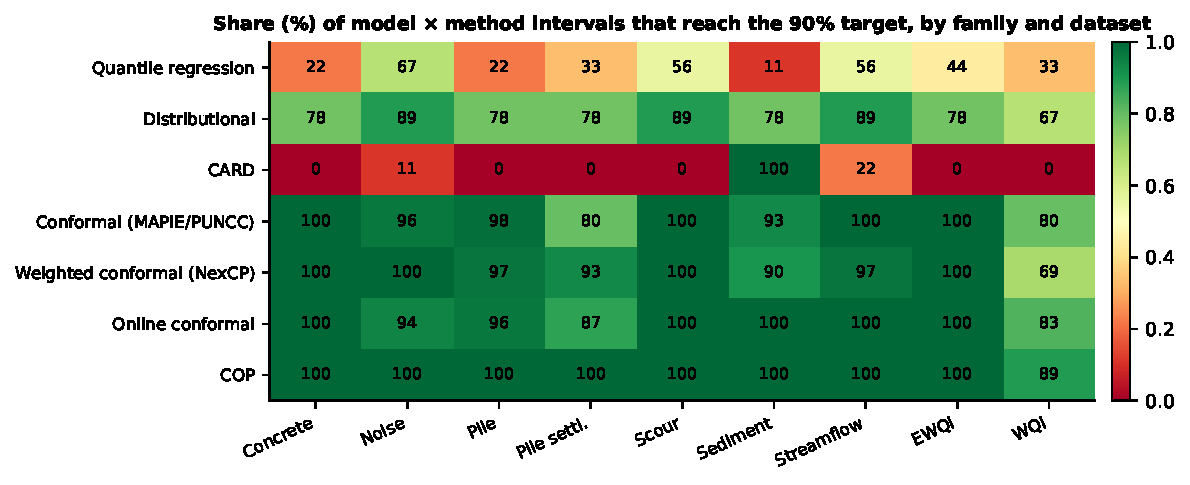
\includegraphics[width=0.95\linewidth]{figures/fig_family_validity.pdf}\caption{Share of model $\times$ method intervals that are valid, by family and dataset.}\label{fig:famvalid}\end{figure}
\begin{figure}[t]\centering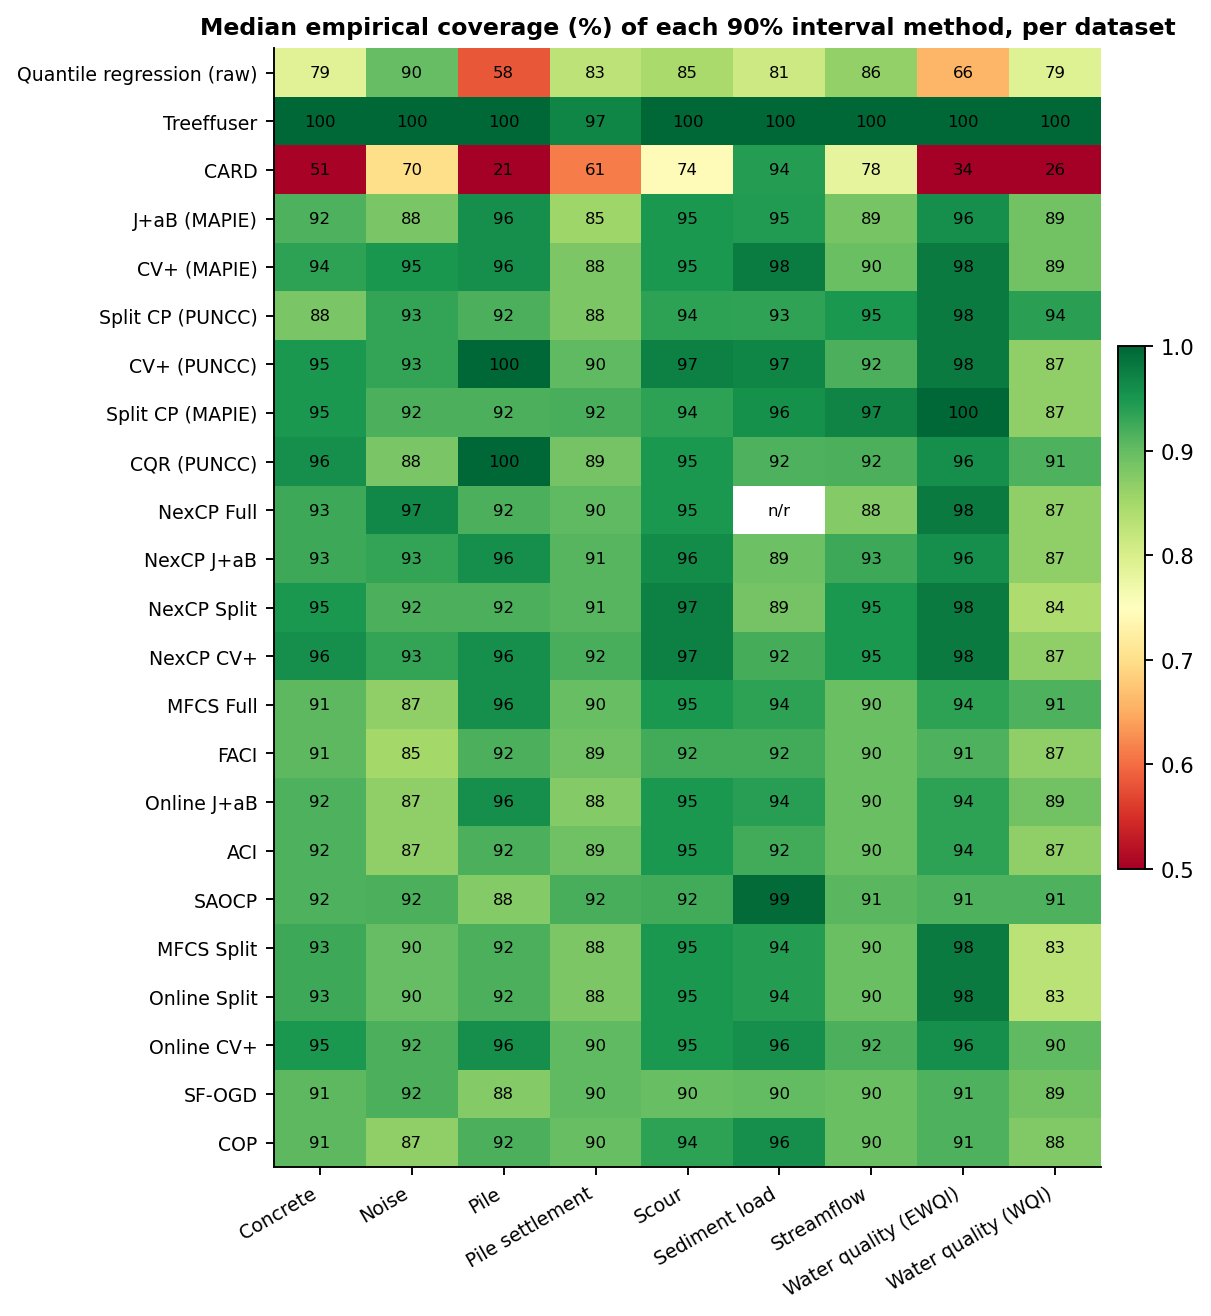
\includegraphics[width=0.9\linewidth]{figures/coverage_heatmap.png}\caption{Median coverage (\%) of every two-sided method on every dataset. n/r: not run.}\label{fig:covheat}\end{figure}
\paragraph{What it shows.}
\begin{itemize}
\item Conformal intervals (MAPIE/PUNCC, NexCP, online, COP) are valid in \textbf{1480 of 1557} cases (95.1\%).
\item The misses concentrate on Water quality (WQI) (37), Pile settlement (21), Noise (7), Sediment load (6), Pile (5), Streamflow (1). WQI has 151 features for 190 training rows, so the out-of-fold
residuals used for calibration come from models fitted on even fewer rows than the final model; pile settlement has a heavy right tail (skewness 2.4), and its few very large
settlements are hard to cover with residuals calibrated mostly on small ones.
\item Model-based families are valid far less often (Table~\ref{tab:family}).
\end{itemize}
\begin{insight}[Takeaway Q2]
On small real datasets the conformal guarantee is not just a theorem: it holds in practice for 95\% of the intervals, and the failures point to the
data (very high dimension, heavy tails), not to the methods.
\end{insight}

\subsection{Q3: the sharpest valid method depends on the data}
\begin{table}[t]\centering\small
\caption{Conformal methods pooled over all datasets and models: number of intervals, datasets, share valid, median relative width, and on how many datasets the method is recommended.}\label{tab:pool}
\begin{tabular}{lrrrrr}\toprule Method & Intervals & Datasets & Valid & Median width/sd & Recommended\\\midrule
J+aB (MAPIE) & 81 & 9 & 91.4\% & 1.27 & 3\\
FACI & 77 & 9 & 96.1\% & 1.29 & 2\\
MFCS Full & 77 & 9 & 100.0\% & 1.32 & 2\\
ACI & 77 & 9 & 97.4\% & 1.32 & 0\\
COP & 77 & 9 & 98.7\% & 1.34 & 0\\
Online J+aB & 77 & 9 & 97.4\% & 1.35 & 0\\
NexCP J+aB & 77 & 9 & 96.1\% & 1.35 & 1\\
CV+ (PUNCC) & 81 & 9 & 95.1\% & 1.40 & 0\\
Online Split & 77 & 9 & 85.7\% & 1.40 & 0\\
MFCS Split & 77 & 9 & 85.7\% & 1.40 & 0\\
Online CV+ & 77 & 9 & 100.0\% & 1.43 & 0\\
Split CP (MAPIE) & 81 & 9 & 91.4\% & 1.44 & 1\\
NexCP Split & 77 & 9 & 89.6\% & 1.45 & 0\\
NexCP Full & 70 & 8 & 91.4\% & 1.47 & 0\\
CV+ (MAPIE) & 81 & 9 & 97.5\% & 1.48 & 0\\
NexCP CV+ & 77 & 9 & 100.0\% & 1.54 & 0\\
SF-OGD & 77 & 9 & 100.0\% & 1.62 & 0\\
SAOCP & 77 & 9 & 98.7\% & 1.64 & 0\\
Split CP (PUNCC) & 81 & 9 & 96.3\% & 1.66 & 0\\
CQR (PUNCC) & 81 & 9 & 92.6\% & 1.77 & 0\\
\bottomrule\end{tabular}\end{table}\begin{table}[t]\centering\small
\caption{Recommended method per dataset: the narrowest method that is valid on at least 75\% of the base models it wraps.}\label{tab:rec}
\begin{tabular}{llrrr}\toprule Dataset & Best model (CV) & Raw QR coverage & Recommended & Coverage / width\\\midrule
Concrete & CatBoost & 79.0\% & MFCS Full & 90.5\% / 1.00\\
Noise & LightGBM & 90.0\% & FACI & 85.0\% / 0.81\\
Pile & LightGBM & 58.3\% & J+aB (MAPIE) & 95.8\% / 1.60\\
Pile settlement & GPBoost & 82.8\% & MFCS Full & 89.8\% / 0.74\\
Scour & XGBoost & 84.6\% & Split CP (MAPIE) & 93.6\% / 1.48\\
Sediment load & TabNet & 81.1\% & NexCP J+aB & 89.3\% / 0.24\\
Streamflow & GradientBoosting & 86.5\% & J+aB (MAPIE) & 88.5\% / 1.32\\
Water quality (EWQI) & XGBoost & 66.0\% & FACI & 91.5\% / 1.33\\
Water quality (WQI) & XGBoost & 79.3\% & J+aB (MAPIE) & 89.0\% / 1.18\\
\bottomrule\end{tabular}\end{table}
\begin{figure}[t]\centering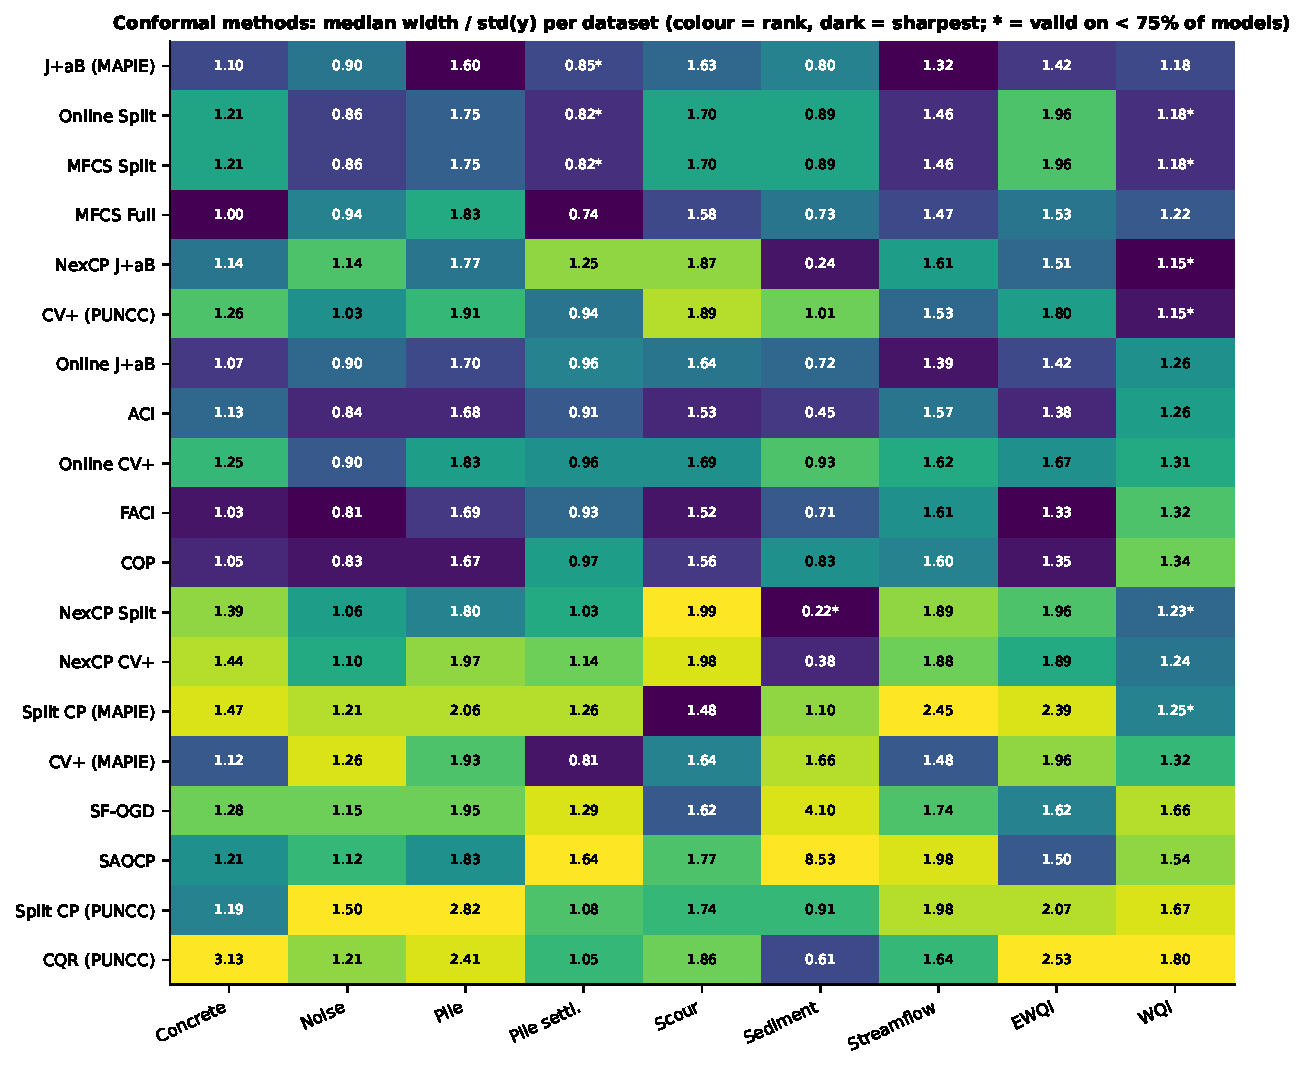
\includegraphics[width=\linewidth]{figures/fig_conformal_ranking.pdf}\caption{Median relative width of each conformal method on each dataset; colour gives the rank within the dataset (dark = sharpest).}\label{fig:rank}\end{figure}
\begin{figure}[t]\centering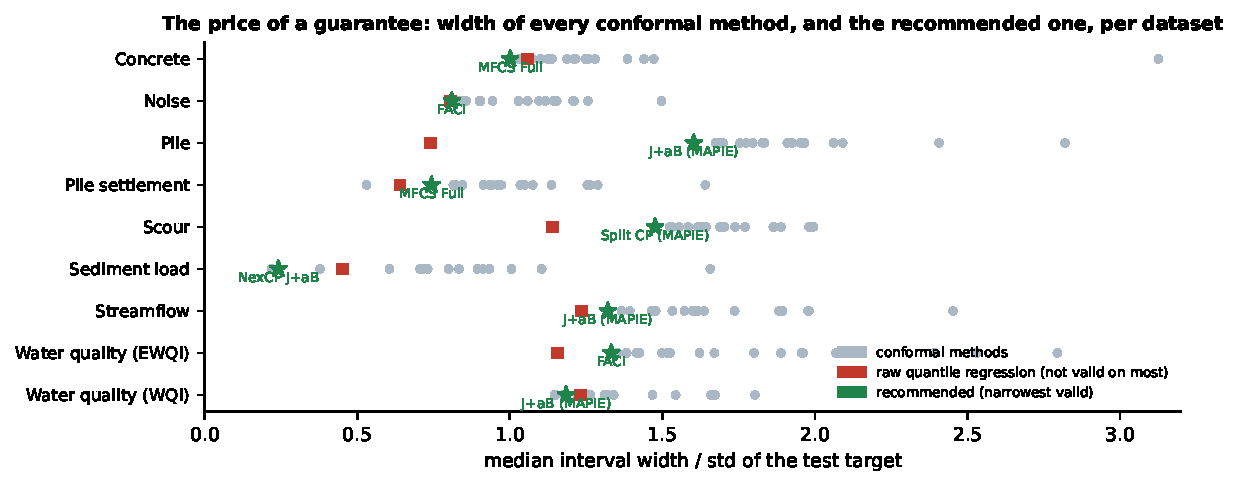
\includegraphics[width=\linewidth]{figures/fig_recommended.pdf}\caption{Relative width of every conformal method (grey), raw quantile regression (red) and the recommended method (star) per dataset.}\label{fig:rec}\end{figure}
\paragraph{What it shows.}
\begin{itemize}
\item Valid methods differ in width by a factor of two or more on the same dataset (Fig.~\ref{fig:rec}).
\item No method is the sharpest everywhere (Fig.~\ref{fig:rank}, Table~\ref{tab:rec}). J+aB (MAPIE) is recommended on 3 datasets; the online
methods FACI and MFCS Full on 4; NexCP J+aB on the large, heavy-tailed sediment data, where recent-weighted residuals adapt to the scale of the target.
\item Jackknife+-after-bootstrap, which reuses every training point for calibration, is usually sharper than split conformal, which calibrates on half the data; CV+ is close to split conformal in width but more often valid.
\item CQR is valid but wide here: with a few hundred points the conformal correction has to repair poorly estimated quantile models.
\end{itemize}
\begin{insight}[Takeaway Q3]
Validity is easy to get; sharpness is not. A practitioner should run a small panel of valid methods (J+aB, CV+, and, if labels arrive sequentially,
FACI or MFCS) and pick the narrowest on held-out data, rather than commit to one method in advance.
\end{insight}

\subsection{Q4: learned coverage and single-network uncertainty}
\begin{table}[t]\centering\small
\caption{Adaptive coverage policies (ACP) and HCM per dataset. Saturated: models whose policy sits at $\tilde\alpha=0.999$; target and coverage are means over the other models.}\label{tab:acphcm}
\resizebox{\textwidth}{!}{\begin{tabular}{lrrrrr}\toprule Dataset & ACP saturated & ACP target & ACP coverage & HCM 95\% cov. & HCM Spearman\\\midrule
Concrete & 0/9 & 63.1\% & 95.6\% & 84.2\% & -0.38\\
Noise & 0/9 & 61.6\% & 89.3\% & 80.0\% & -0.12\\
Pile & 0/9 & 82.1\% & 100.0\% & 100.0\% & -0.00\\
Pile settlement & 0/9 & 63.2\% & 82.7\% & 86.6\% & 0.51\\
Scour & 0/9 & 87.1\% & 100.0\% & 91.0\% & -0.11\\
Sediment load & 9/9 & -- & -- & 100.0\% & -0.57\\
Streamflow & 9/9 & -- & -- & 95.8\% & -0.15\\
Water quality (EWQI) & 4/9 & 5.4\% & 60.0\% & 97.9\% & 0.31\\
Water quality (WQI) & 0/9 & 22.8\% & 54.3\% & 81.7\% & 0.30\\
\bottomrule\end{tabular}}\end{table}
\begin{figure}[t]\centering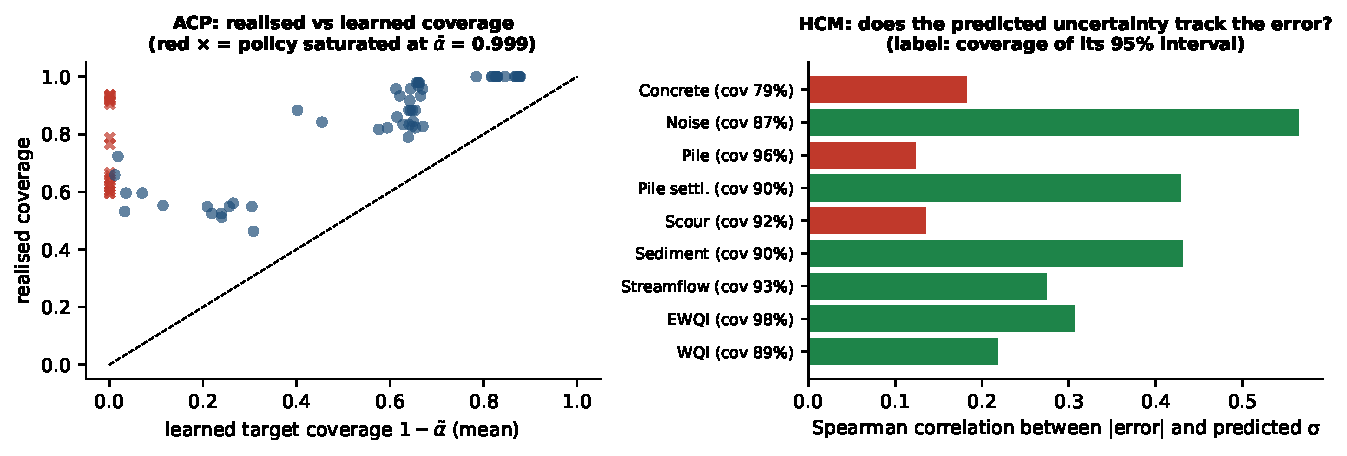
\includegraphics[width=\linewidth]{figures/fig_acp_hcm.pdf}\caption{Left: ACP realised coverage against its learned target. Right: HCM's Spearman correlation between absolute error and predicted spread.}\label{fig:acphcm}\end{figure}
ACP's guarantee is relative to its own learned level, and its realised coverage is always above that level (Fig.~\ref{fig:acphcm}, left). On
sediment load and streamflow, and for four models on EWQI, the policy saturated at $\tilde\alpha=0.999$: the learned level then carries no information and
every set has the same width. HCM's 95\% interval covers 80--100\%, but its predicted spread is negatively correlated with the error, or not at all, on six of
nine datasets (Fig.~\ref{fig:acphcm}, right), so on these small tabular problems a single network does not know when it is wrong.

\section{Discussion}\label{sec:discussion}
\paragraph{A practical recipe.} (1) Tune the base model by cross-validation only. (2) Wrap it in jackknife+-after-bootstrap or CV+; these are valid
on almost every dataset and model here and need no extra data. (3) If labels arrive one at a time, add an online method (FACI, MFCS) and let it adapt.
(4) Check coverage against the sample-size threshold of eq.~\eqref{eq:valid}, not against exactly 90\%. (5) Use predictive distributions for their CRPS
and shape, not for their raw intervals, unless they are conformalised.
\paragraph{When the guarantee bends.} The two datasets with most conformal misses share a feature: the calibration residuals do not represent the test
residuals (too few rows per feature on WQI; a heavy right tail on pile settlement). Weighted (NexCP) and online methods are designed for
exactly this, and they recover coverage on pile settlement (MFCS Full is recommended there).

\paragraph{Limitations and threats to validity.}
\begin{itemize}
\item \textbf{One split, one run.} Every number comes from one fixed train/test split and one run, so coverages carry the sampling
error of~\eqref{eq:valid} and no confidence intervals across splits or seeds are available. Small test sets (fewer than 100 points)
can only distinguish large departures from 90\%.
\item \textbf{Order of the test set.} Online methods depend on the order of the stored test rows, which has no time meaning on most
datasets; their good widths partly reflect learning from earlier test labels.
\item \textbf{Marginal, not conditional.} All guarantees are marginal. A method can cover 90\% overall and much less for large target
values; the interval figures show where misses concentrate.
\item \textbf{Approximate tuning reproducibility.} Optuna search is not bit-reproducible; the stored tuning run is the one every
later notebook used. CARD, TabNet, HCM and ACP are neural and depend on their seeds.
\item \textbf{Compute limits.} Kaggle stops a session after 12 hours. Jobs that did not finish are listed as not run; their methods are
missing from the tables rather than estimated.
\end{itemize}

\section{Future work: the \texttt{reguq} library}\label{sec:future}
The notebooks are a research pipeline: they are long, dataset-specific copies of one another, and their methods cannot be imported
into other code. The next step of this project is a Python package, \textbf{\texttt{reguq}} (regression uncertainty quantification),
that turns the verified methods of this benchmark into a tested, documented library:
\begin{itemize}
\item one interface, \texttt{fit / calibrate / predict\_interval / predict\_distribution}, for every family studied here (quantile
regression, distributional models, split/cross/bootstrap conformal, NexCP, online conformal, Extreme CP, ACP, HCM), wrapping any
scikit-learn-style regressor;
\item the evaluation protocol of Section~\ref{sec:eval} (coverage with its sampling tolerance, relative width, CRPS, PIT, crossing
rate) and the recommendation rule as functions, so that a new dataset can be benchmarked in a few lines;
\item unit tests that check each method against the authors' reference code and against its theoretical coverage on synthetic data;
\item repeated random splits and confidence intervals for coverage and width, which the notebooks do not provide, and conditional
coverage diagnostics (coverage by target range and by feature bins).
\end{itemize}

\section{Conclusions}
\begin{itemize}
\item Raw quantile regression and native Gaussian predictive distributions do not deliver their nominal 90\% coverage on these datasets.
\item Conformal methods are valid in 1480 of 1557 cases; their failures are explained by the data.
\item The sharpest valid method depends on the dataset; J+aB, FACI, MFCS Full, NexCP J+aB and split conformal are each recommended at least once.
\item Learned-coverage policies can saturate, and single-network uncertainty is not reliably informative on small tabular data.
\end{itemize}
\paragraph{Per-dataset reports.} \texttt{papers/<dataset>/paper.pdf} for Concrete, Noise, Pile, Pile settlement, Scour, Sediment load, Streamflow, Water quality (EWQI), Water quality (WQI).
\paragraph{Reproducibility.} Code, executed notebooks and raw outputs: \url{https://github.com/DaneshSelwal/Regression_Uncertainty_Quantification_Analysis} (branch \texttt{version2.0}). Machine-readable results:
\texttt{results/benchmark\_long.csv} (every interval), \texttt{benchmark\_methods.csv}, \texttt{benchmark\_datasets.csv}. Every Kaggle run is listed in
\texttt{docs/run\_registry.tsv} and in each dataset's report.
\paragraph{Acknowledgements.} Computations were run on Kaggle's free CPU sessions.
\FloatBarrier
\bibliographystyle{plainnat}\bibliography{references}
\end{document}
